%**************************************************************************************
% License:
% CC BY-NC-SA 4.0 (http://creativecommons.org/licenses/by-nc-sa/4.0/)
%**************************************************************************************

\documentclass[notes]{beamer}

\mode<presentation> {

\usetheme{Madrid}

% Burnt orange
\definecolor{burntorange}{rgb}{0.8, 0.33, 0.0}
\colorlet{beamer@blendedblue}{burntorange}
% Pale yellow
\definecolor{paleyellow}{rgb}{1.0, 1.0, 0.953}
\setbeamercolor{background canvas}{bg=white}
% Secondary and tertiary palette
\setbeamercolor*{palette secondary}{use=structure,fg=white,bg=burntorange!80!black}
\setbeamercolor*{palette tertiary}{use=structure,fg=white,bg=burntorange!60!black}

% To remove the navigation symbols from the bottom of all slides uncomment this line
%\setbeamertemplate{navigation symbols}{}
}

\usepackage{amsmath}
\DeclareMathOperator*{\argmin}{arg\,min}
\DeclareMathOperator*{\argmax}{arg\,max}
\usepackage{bm}
\usepackage{booktabs}
\usepackage{breqn}
\usepackage{cleveref}
\usepackage{graphicx}
\usepackage[labelsep=space,tableposition=top]{caption}
\renewcommand{\figurename}{Fig.}
\usepackage{caption,subcaption}
\usepackage{xcolor}
\usepackage{verbatim}
\usepackage{tikz}
\usetikzlibrary{shapes,arrows,positioning,calc}

%----------------------------------------------------------------------------------------
%	TITLE PAGE
%----------------------------------------------------------------------------------------
\title[LSTM for Liquefaction]{Long Short-Term Memory Networks for Predicting Pore Pressure in Liquefaction}
\author{Krishna Kumar \& Ellen Rathje}
\institute[UT Austin]
{
University of Texas at Austin \\
\medskip
}
\date{}

\begin{document}

\begin{frame}
\titlepage
\end{frame}

\begin{frame}
 \frametitle{Overview}
 \tableofcontents
\end{frame}

%----------------------------------------------------------------------------------------
% SLIDES
%----------------------------------------------------------------------------------------

%------------------------------------------------
\section{The Liquefaction Problem}
%------------------------------------------------

\begin{frame}
\frametitle{What is Liquefaction?}

\begin{figure}
\centering
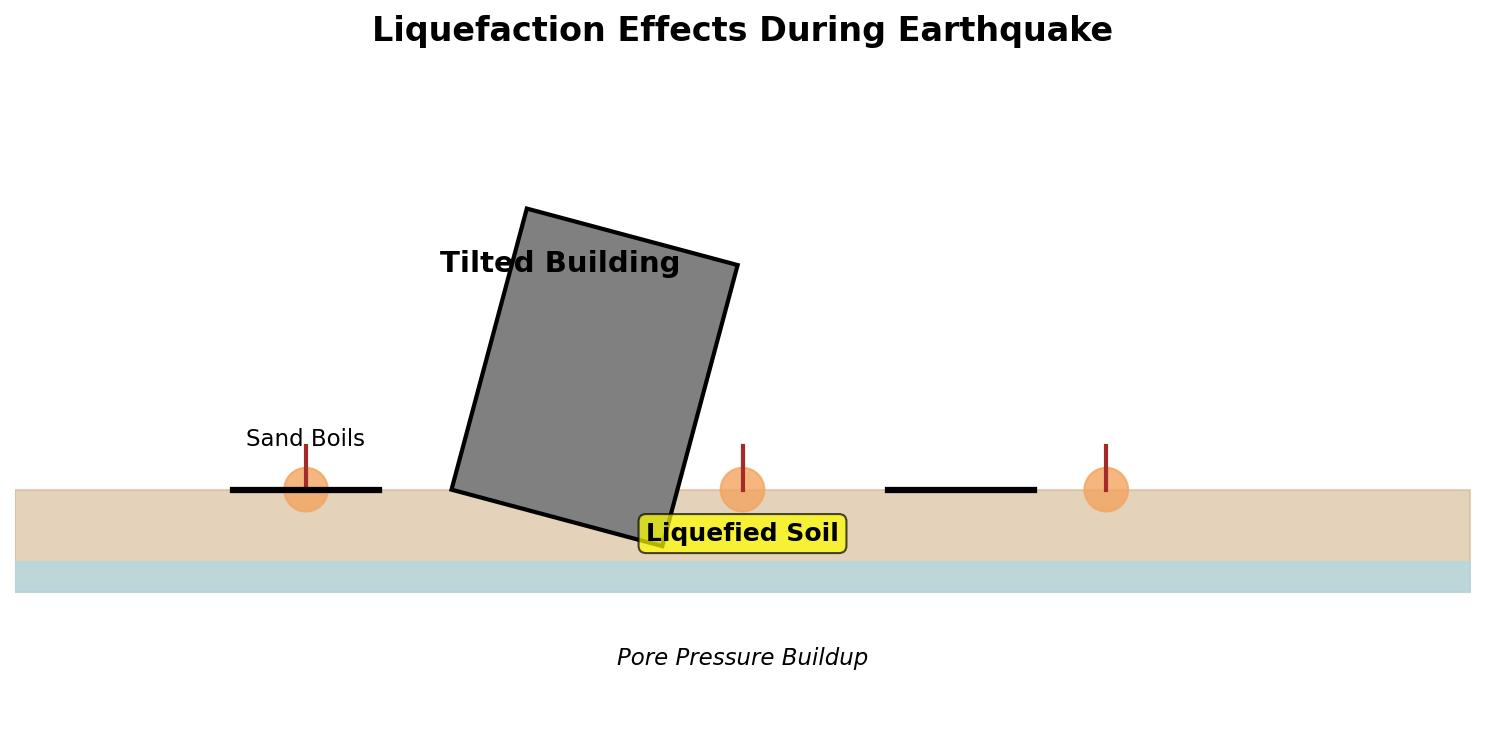
\includegraphics[width=0.75\textwidth]{figs/liquefaction_damage.jpg}
\caption{Liquefaction damage during earthquake}
\end{figure}

\mode<beamer>{
\textbf{Definition:} Saturated soil loses strength during cyclic loading (earthquakes)

\vspace{0.5em}

\textbf{Consequences:}
\begin{itemize}
\item Building settlements and tilting
\item Bridge foundation failures
\item Lateral spreading
\end{itemize}
}
\mode<handout>{
\vspace{2cm}
}

\end{frame}

%------------------------------------------------
\begin{frame}
\frametitle{The Physics: Pore Pressure Buildup}

\textbf{Effective Stress Principle:}
\begin{equation}
\sigma' = \sigma - u
\end{equation}

where $\sigma'$ = effective stress, $\sigma$ = total stress, $u$ = pore water pressure

\vspace{0.5em}

\textbf{Pore Pressure Ratio:}
\begin{equation}
r_u = \frac{u_{excess}}{\sigma'_0}
\end{equation}

\mode<beamer>{
\textbf{Liquefaction occurs when:} $r_u \geq 1.0$

\vspace{1em}

\begin{figure}
\centering
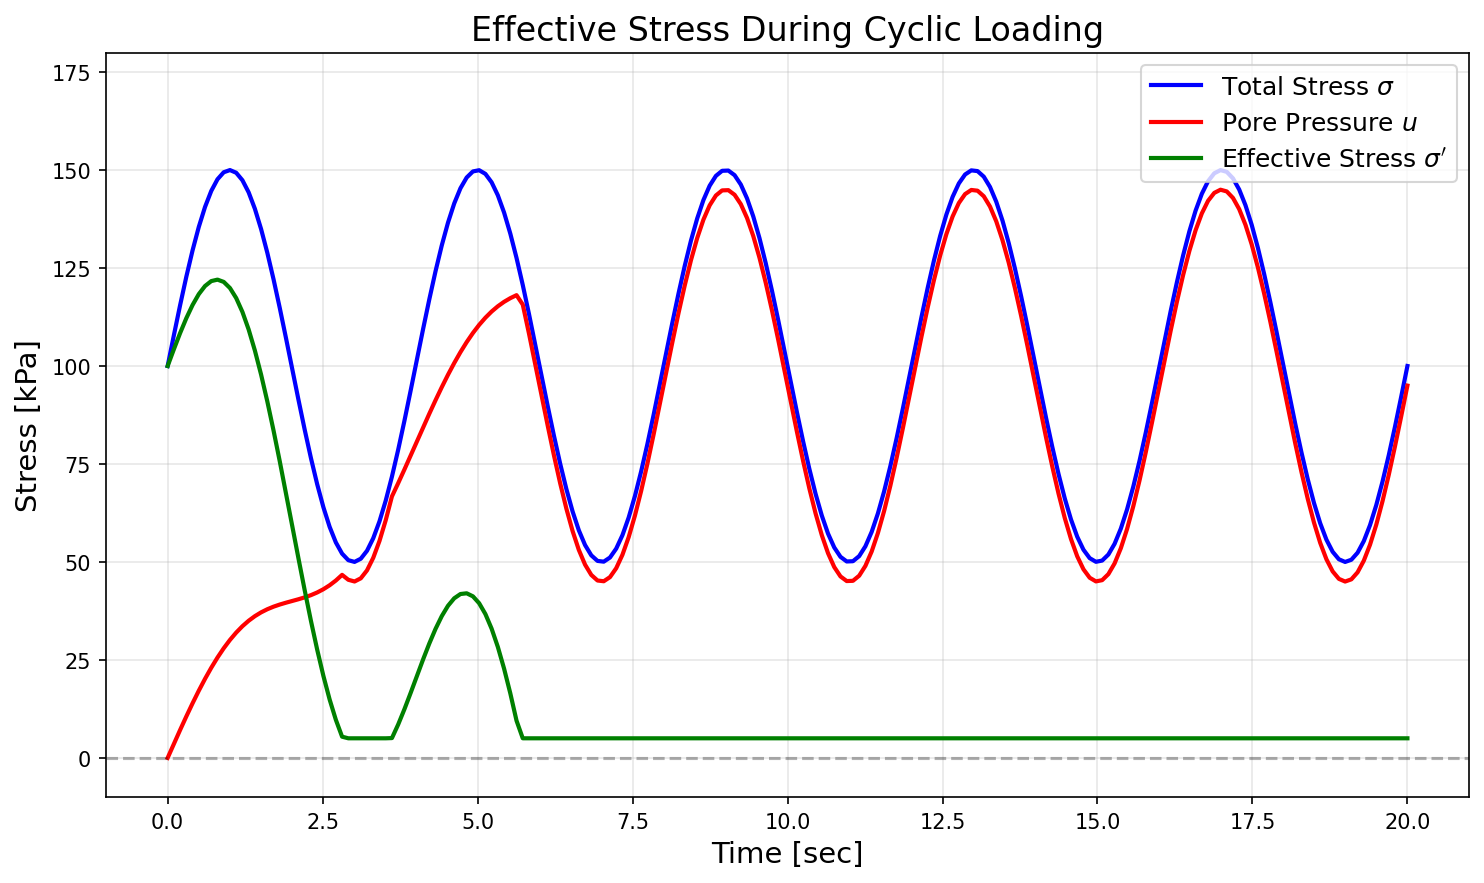
\includegraphics[width=0.5\textwidth]{figs/effective_stress.png}
\caption{Effective stress during cyclic loading}
\end{figure}
}
\mode<handout>{
\vspace{3cm}
}

\end{frame}

%------------------------------------------------
\begin{frame}
\frametitle{The Challenge: Stress History Dependency}

\textbf{Key Observation:} Pore pressure generation depends on \textbf{entire stress history}, not just current stress!

\vspace{0.5em}

\mode<beamer>{
\textbf{The Shielding Effect:}
\begin{itemize}
\item When current shear stress amplitude $<$ prior peak amplitude
\item Pore pressure remains nearly constant ("shielded")
\item Sophisticated constitutive models (PM4Sand, PDMY02) \textbf{fail} to capture this
\end{itemize}

\vspace{0.5em}

\begin{center}
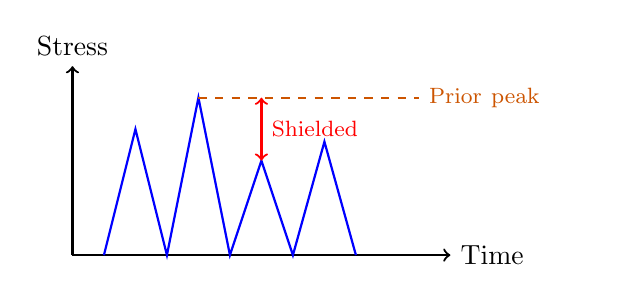
\begin{tikzpicture}[scale=0.8]
    \draw[->,thick] (0,0) -- (6,0) node[right] {Time};
    \draw[->,thick] (0,0) -- (0,3) node[above] {Stress};

    % Stress amplitude
    \draw[blue,thick] (0.5,0) -- (1,2) -- (1.5,0) -- (2,2.5) -- (2.5,0) -- (3,1.5) -- (3.5,0) -- (4,1.8) -- (4.5,0);

    % Peak marker
    \draw[burntorange,dashed,thick] (2,2.5) -- (5.5,2.5) node[right,text width=2cm] {\footnotesize Prior peak};

    % Shielding region
    \draw[red,thick,<->] (3,1.5) -- (3,2.5) node[midway,right] {\footnotesize Shielded};
\end{tikzpicture}
\end{center}
}
\mode<handout>{
\vspace{3cm}
}

\end{frame}

%------------------------------------------------
\section{Traditional Approaches Fail}
%------------------------------------------------

\begin{frame}
\frametitle{Limitations of Constitutive Models}

\textbf{Common Models:} PM4Sand, PDMY02, Dafalias-Manzari

\vspace{0.5em}

\mode<beamer>{
\textbf{Problems:}
\begin{enumerate}
\item Cannot capture shielding effect
\item Predict continuous pore pressure increase
\item Miss stress history dependencies
\item Poor predictions of liquefaction timing
\item Require extensive calibration (15-30+ parameters)
\end{enumerate}

\vspace{1em}

\textbf{Why Simple Neural Networks Fail Too:}
\begin{itemize}
\item Take current state as input: $y_t = f(x_t)$
\item \textbf{No memory} of past events
\item Cannot learn temporal dependencies
\end{itemize}

\vspace{0.5em}

\textbf{What We Need:} $y_t = f(x_t, x_{t-1}, x_{t-2}, \ldots, x_0)$
}
\mode<handout>{
\vspace{4cm}
}

\end{frame}

%------------------------------------------------
\section{Sequence Models: RNNs}
%------------------------------------------------

\begin{frame}
\frametitle{From Feedforward to Recurrent Networks}

\begin{columns}[T]
\column{0.5\textwidth}
\textbf{Feedforward Neural Network:}
\begin{center}
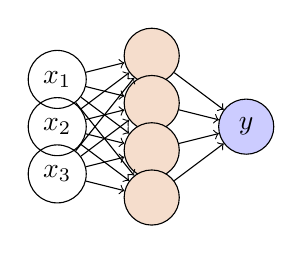
\begin{tikzpicture}[scale=0.6]
    % Input layer
    \foreach \i in {1,2,3} {
        \node[circle,draw,minimum size=0.7cm] (i\i) at (0,-\i) {$x_\i$};
    }
    % Hidden layer
    \foreach \i in {1,2,3,4} {
        \node[circle,draw,minimum size=0.7cm,fill=burntorange!20] (h\i) at (2,-\i+0.5) {};
    }
    % Output layer
    \node[circle,draw,minimum size=0.7cm,fill=blue!20] (o1) at (4,-2) {$y$};

    % Connections
    \foreach \i in {1,2,3} {
        \foreach \j in {1,2,3,4} {
            \draw[->,thin] (i\i) -- (h\j);
        }
    }
    \foreach \i in {1,2,3,4} {
        \draw[->,thin] (h\i) -- (o1);
    }
\end{tikzpicture}
\end{center}
No memory, fixed input size

\column{0.5\textwidth}
\textbf{Recurrent Neural Network:}
\begin{center}
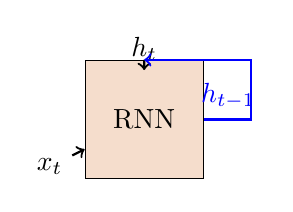
\begin{tikzpicture}[scale=0.6]
    % RNN cell
    \node[rectangle,draw,minimum width=1.5cm,minimum height=1.5cm,fill=burntorange!20] (rnn) at (2,0) {RNN};

    % Input
    \node (x) at (0,-1) {$x_t$};
    \draw[->,thick] (x) -- (rnn);

    % Output
    \node (y) at (2,1.5) {$h_t$};
    \draw[->,thick] (rnn) -- (y);

    % Recurrent connection
    \draw[->,thick,blue] (rnn.east) -- ++(1,0) |- (rnn.north);
    \node[right] at (3,0.5) {\color{blue} $h_{t-1}$};
\end{tikzpicture}
\end{center}
Loops allow information persistence
\end{columns}

\vspace{0.5em}

\textbf{RNN Equation:}
\begin{equation}
h_t = \tanh(W_{xh} x_t + W_{hh} h_{t-1} + b_h)
\end{equation}

\end{frame}

%------------------------------------------------
\begin{frame}
\frametitle{The Vanishing Gradient Problem}

\textbf{Problem with RNNs:}

\mode<beamer>{
\begin{itemize}
\item Gradients multiplied many times during backpropagation
\item Gradients vanish ($\to 0$) or explode ($\to \infty$)
\item Cannot learn long-term dependencies
\end{itemize}

\vspace{0.5em}

\begin{equation}
\frac{\partial L}{\partial W} = \prod_{t=1}^{T} \frac{\partial h_t}{\partial h_{t-1}} \frac{\partial h_t}{\partial W}
\end{equation}

If $\left|\frac{\partial h_t}{\partial h_{t-1}}\right| < 1$: gradient $\to 0$ as $T \to \infty$

\vspace{1em}

\textbf{Impact:} Can't remember events 10+ steps ago

\textbf{For liquefaction:} Need to remember 100s-1000s of loading cycles!

\vspace{0.5em}

\begin{figure}
\centering
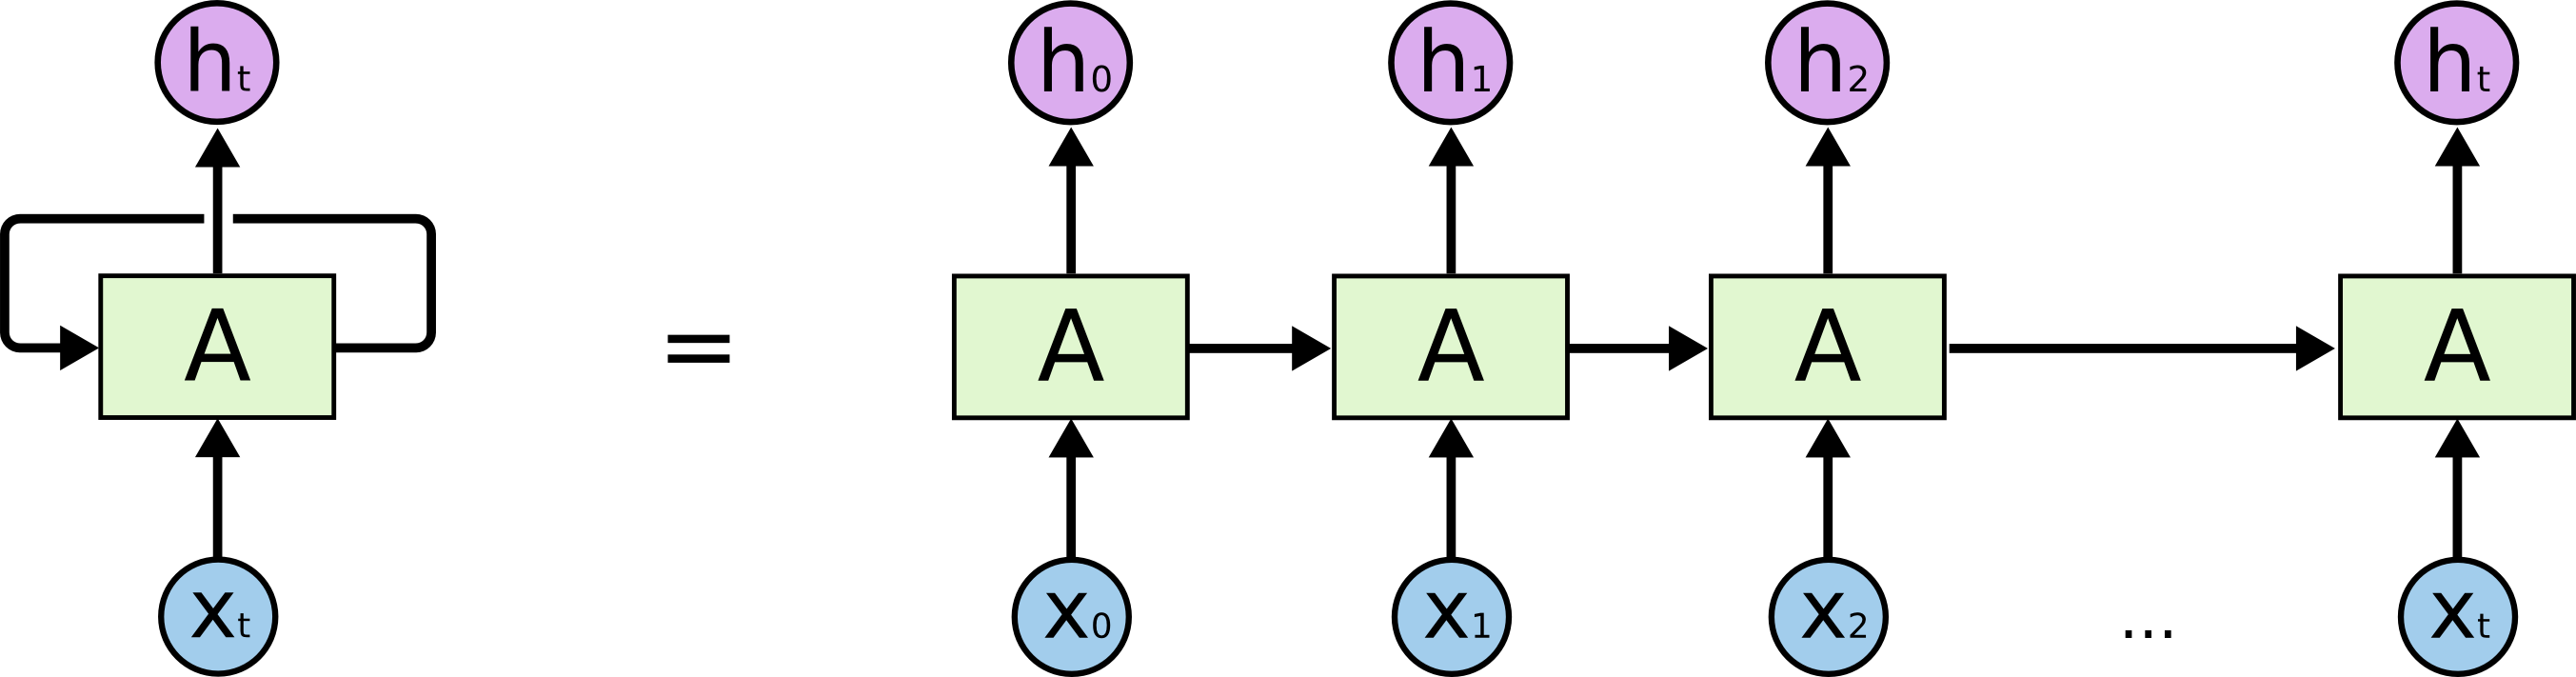
\includegraphics[width=0.5\textwidth]{figs/vanishing_gradient.png}
\caption{Gradient magnitude decays exponentially}
\end{figure}
}
\mode<handout>{
\vspace{4cm}
}

\end{frame}

%------------------------------------------------
\begin{frame}
\frametitle{Sequence-to-Sequence Learning}

\textbf{General Framework:} Map input sequence $\to$ output sequence

\vspace{0.5em}

\begin{center}
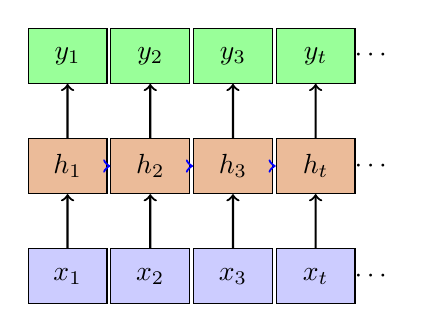
\begin{tikzpicture}[scale=0.7]
    % Input sequence
    \foreach \i/\label in {1/$x_1$,2/$x_2$,3/$x_3$,4/$x_t$} {
        \node[rectangle,draw,fill=blue!20,minimum width=1cm,minimum height=0.7cm] (x\i) at (\i*1.5,0) {\label};
    }

    % RNN cells
    \foreach \i/\label in {1/$h_1$,2/$h_2$,3/$h_3$,4/$h_t$} {
        \node[rectangle,draw,fill=burntorange!40,minimum width=1cm,minimum height=0.7cm] (h\i) at (\i*1.5,2) {\label};
    }

    % Output sequence
    \foreach \i/\label in {1/$y_1$,2/$y_2$,3/$y_3$,4/$y_t$} {
        \node[rectangle,draw,fill=green!40,minimum width=1cm,minimum height=0.7cm] (y\i) at (\i*1.5,4) {\label};
    }

    % Connections
    \foreach \i in {1,2,3,4} {
        \draw[->,thick] (x\i) -- (h\i);
        \draw[->,thick] (h\i) -- (y\i);
    }

    % Recurrent connections
    \foreach \i in {1,2,3} {
        \pgfmathtruncatemacro{\j}{\i+1}
        \draw[->,thick,blue] (h\i) -- (h\j);
    }

    \node at (7,0) {$\cdots$};
    \node at (7,2) {$\cdots$};
    \node at (7,4) {$\cdots$};
\end{tikzpicture}
\end{center}

\mode<beamer>{
\textbf{For Liquefaction:}
\begin{itemize}
\item \textbf{Input sequence:} Stress history $[\tau_1, \tau_2, \ldots, \tau_t]$
\item \textbf{Output:} Pore pressure ratio $r_u(t)$
\item Use sliding window (window = 800 timesteps $\approx$ 2 cycles)
\end{itemize}
}
\mode<handout>{
\vspace{2cm}
}

\end{frame}

%------------------------------------------------
\section{LSTM: The Solution}
%------------------------------------------------

\begin{frame}
\frametitle{Long Short-Term Memory (LSTM)}

\textbf{Key Innovation:} Replace simple RNN cell with complex \textbf{memory cell}

\vspace{0.5em}

\mode<beamer>{
\textbf{Developed by:} Hochreiter \& Schmidhuber (1997)

\vspace{0.5em}

\textbf{LSTM Can:}
\begin{enumerate}
\item \textbf{Remember} information for long periods
\item \textbf{Forget} irrelevant information
\item \textbf{Selectively update} memory
\end{enumerate}

\vspace{0.5em}

\textbf{Applications:}
\begin{itemize}
\item Machine translation
\item Speech recognition
\item Time series forecasting
\item \textbf{Now: Geotechnical engineering!}
\end{itemize}

\vspace{0.5em}

\begin{figure}
\centering
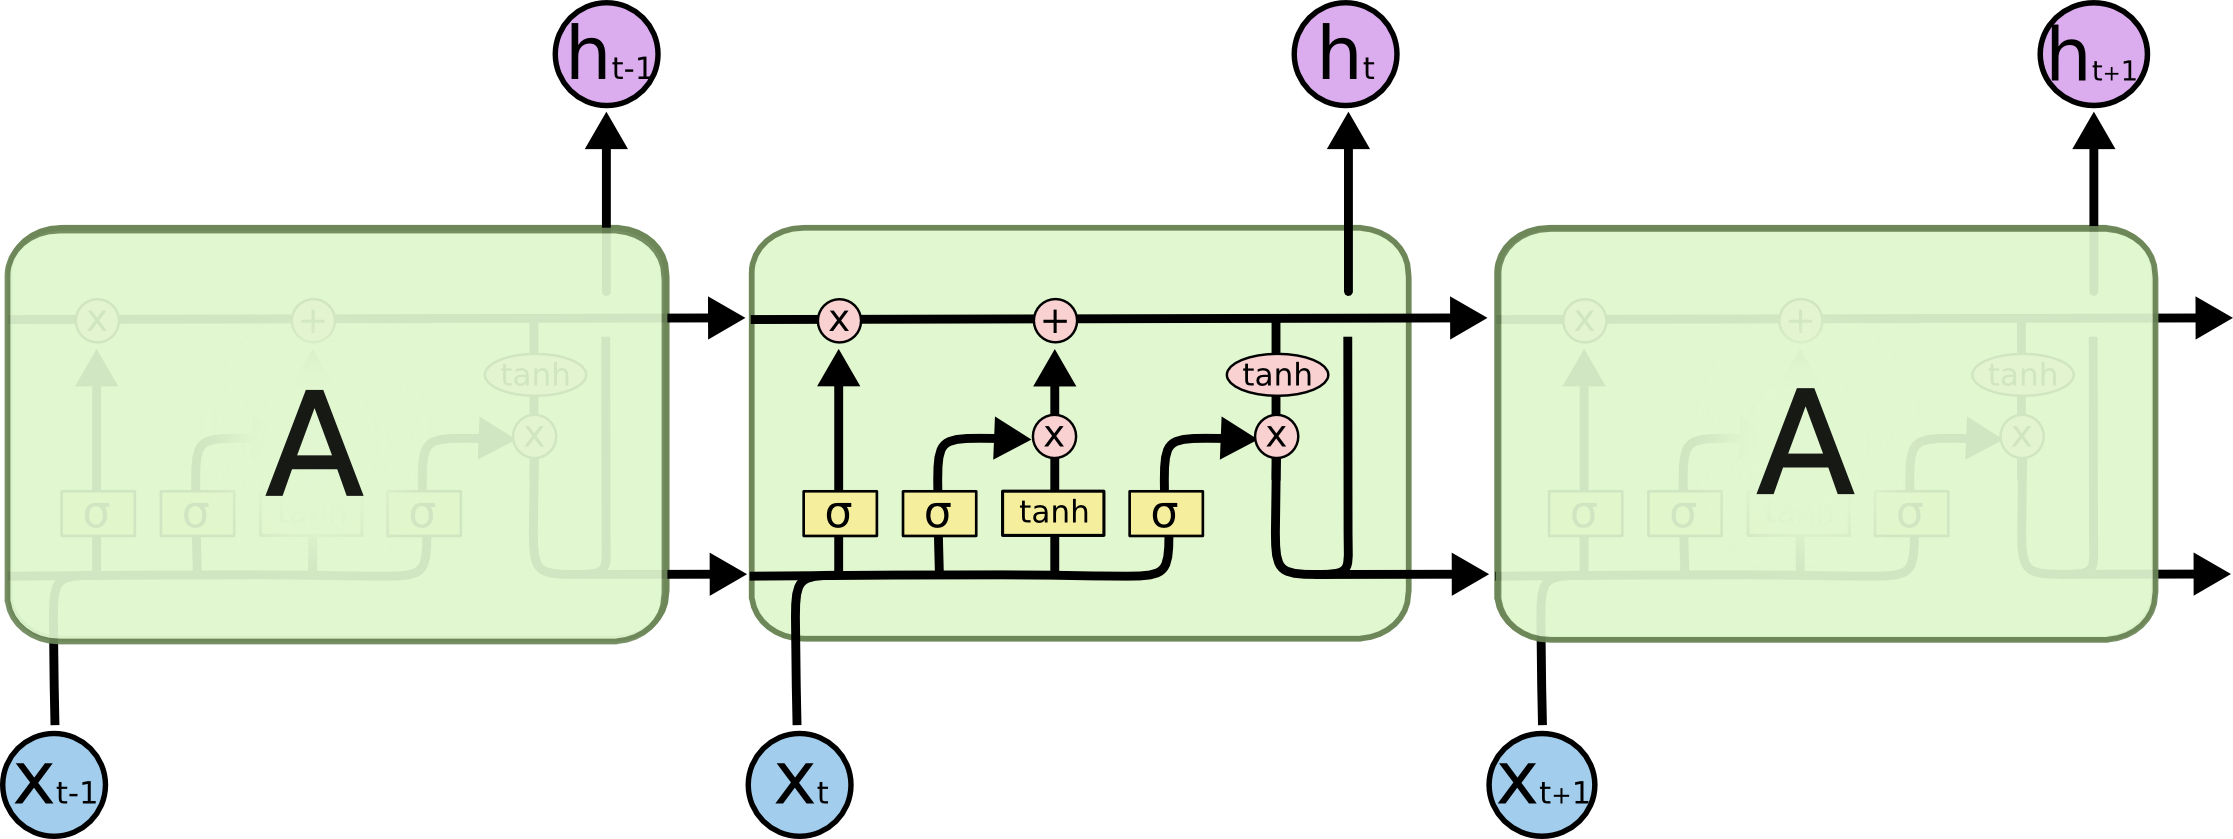
\includegraphics[width=0.5\textwidth]{figs/lstm_overview.png}
\caption{LSTM maintains constant gradient flow via cell state}
\end{figure}
}
\mode<handout>{
\vspace{4cm}
}

\end{frame}

%------------------------------------------------
\begin{frame}
\frametitle{LSTM Architecture: The Three Gates}

\begin{center}
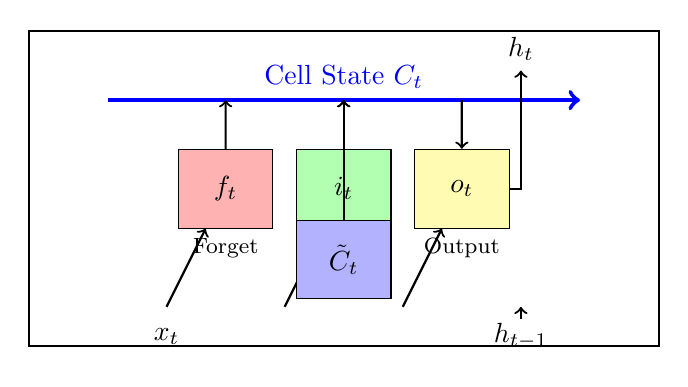
\begin{tikzpicture}[scale=0.75]
    % Main cell
    \node[rectangle,draw,thick,minimum width=8cm,minimum height=4cm] (cell) at (0,0) {};

    % Cell state line
    \draw[->,ultra thick,blue] (-4,1.5) -- (4,1.5) node[above,midway] {Cell State $C_t$};

    % Forget gate
    \node[rectangle,draw,fill=red!30,minimum width=1.2cm,minimum height=1cm] (forget) at (-2,0) {$f_t$};
    \node[below] at (forget.south) {\footnotesize Forget};
    \draw[->,thick] (-3,-2) -- (forget);
    \draw[->,thick] (forget) -- (-2,1.5);

    % Input gate
    \node[rectangle,draw,fill=green!30,minimum width=1.2cm,minimum height=1cm] (input) at (0,0) {$i_t$};
    \node[below] at (input.south) {\footnotesize Input};
    \draw[->,thick] (-1,-2) -- (input);
    \draw[->,thick] (input) -- (0,1.5);

    % Cell update
    \node[rectangle,draw,fill=blue!30,minimum width=1.2cm,minimum height=1cm] (update) at (0,-1.2) {$\tilde{C}_t$};
    \draw[->,thick] (update) -- (0,1.5);

    % Output gate
    \node[rectangle,draw,fill=yellow!30,minimum width=1.2cm,minimum height=1cm] (output) at (2,0) {$o_t$};
    \node[below] at (output.south) {\footnotesize Output};
    \draw[->,thick] (1,-2) -- (output);
    \draw[->,thick] (2,1.5) -- (output);
    \draw[->,thick] (output) -- (3,0) -- (3,2) node[above] {$h_t$};

    % Input/hidden from previous
    \node at (-3,-2.5) {$x_t$};
    \node at (3,-2.5) {$h_{t-1}$};
    \draw[->,thick] (3,-2.2) -- (3,-2);
\end{tikzpicture}
\end{center}

\mode<beamer>{
\textbf{Three gates control information flow:}
\begin{enumerate}
\item \textcolor{red}{Forget gate} $f_t$: What to remove from memory
\item \textcolor{green!50!black}{Input gate} $i_t$: What new info to store
\item \textcolor{yellow!50!black}{Output gate} $o_t$: What to output now
\end{enumerate}
}
\mode<handout>{
\vspace{1cm}
}

\end{frame}

%------------------------------------------------
\begin{frame}
\frametitle{LSTM Mathematics: Gate Equations}

\textbf{Input:} $x_t$ (current), $h_{t-1}$ (previous hidden), $C_{t-1}$ (previous cell state)

\vspace{0.5em}

\mode<beamer>{
\textbf{1. Forget Gate} (what to discard):
\begin{equation}
f_t = \sigma(W_f \cdot [h_{t-1}, x_t] + b_f)
\end{equation}

\textbf{2. Input Gate} (what to add):
\begin{equation}
i_t = \sigma(W_i \cdot [h_{t-1}, x_t] + b_i)
\end{equation}

\textbf{3. Candidate Cell State}:
\begin{equation}
\tilde{C}_t = \tanh(W_C \cdot [h_{t-1}, x_t] + b_C)
\end{equation}

\vspace{0.5em}

Where: $\sigma$ = sigmoid (outputs 0 to 1), $\tanh$ = hyperbolic tangent (outputs -1 to 1)
}
\mode<handout>{
\vspace{3cm}
}

\end{frame}

%------------------------------------------------
\begin{frame}
\frametitle{LSTM Mathematics: State Updates}

\textbf{4. Update Cell State:}
\begin{equation}
C_t = f_t \odot C_{t-1} + i_t \odot \tilde{C}_t
\end{equation}

\mode<beamer>{
\begin{itemize}
\item $f_t \odot C_{t-1}$: Forget old information
\item $i_t \odot \tilde{C}_t$: Add new information
\item $\odot$: Element-wise multiplication
\end{itemize}

\vspace{0.5em}

\textbf{5. Output Gate:}
\begin{equation}
o_t = \sigma(W_o \cdot [h_{t-1}, x_t] + b_o)
\end{equation}

\textbf{6. Hidden State:}
\begin{equation}
h_t = o_t \odot \tanh(C_t)
\end{equation}

\vspace{0.5em}

\textbf{Key Point:} Cell state $C_t$ flows with minimal modification $\to$ solves vanishing gradient!
}
\mode<handout>{
\vspace{3cm}
}

\end{frame}

%------------------------------------------------
\begin{frame}
\frametitle{Why LSTM Solves Vanishing Gradients}

\textbf{Regular RNN:}
\begin{itemize}
\item Gradient flows through $\tanh$ repeatedly
\item After $T$ steps: gradient $\approx 0$
\end{itemize}

\vspace{0.5em}

\textbf{LSTM:}
\begin{itemize}
\item Cell state provides \textbf{highway} for gradients
\item Additive updates preserve gradient
\end{itemize}

\begin{equation}
C_t = f_t \odot C_{t-1} + i_t \odot \tilde{C}_t
\end{equation}

\mode<beamer>{
\vspace{1em}

\textbf{Analogy:} LSTM is like a smart notebook
\begin{itemize}
\item \textcolor{red}{Forget gate}: Eraser (remove old notes)
\item \textcolor{green!50!black}{Input gate}: Pen filter (decide what to write)
\item \textcolor{yellow!50!black}{Output gate}: Cover (control what readers see)
\end{itemize}

\vspace{0.5em}

\begin{figure}
\centering
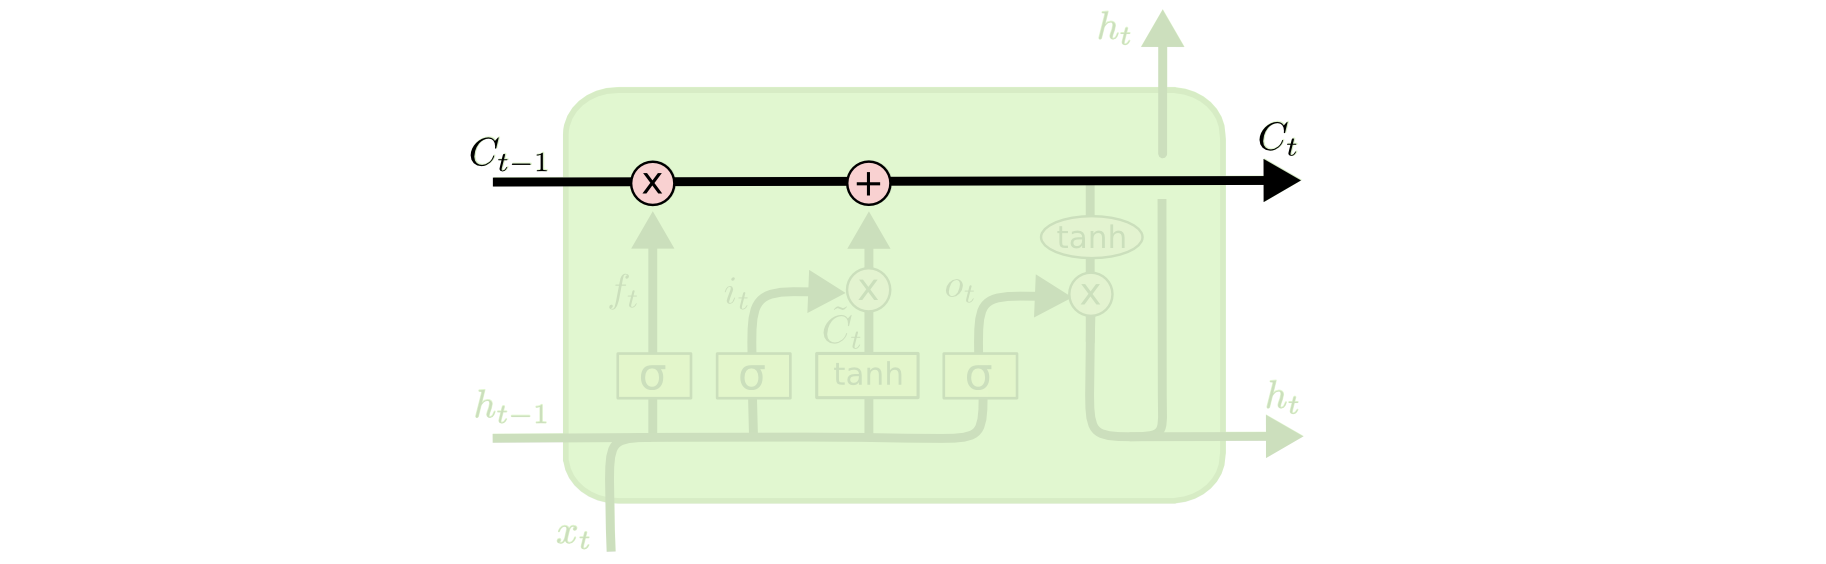
\includegraphics[width=0.5\textwidth]{figs/gradient_flow.png}
\caption{Cell state acts as gradient highway}
\end{figure}
}
\mode<handout>{
\vspace{3cm}
}

\end{frame}

%------------------------------------------------
\section{LSTM for Liquefaction}
%------------------------------------------------

\begin{frame}
\frametitle{Problem Formulation}

\textbf{Goal:} Predict pore pressure ratio $r_u(t)$ from stress history

\vspace{0.5em}

\mode<beamer>{
\textbf{Input Features:}
\begin{enumerate}
\item Normalized time: $T_{\text{norm}} = t/t_{\text{final}}$
\item Normalized shear stress: $\tau_{\text{norm}} = \tau/\sigma'_0$
\item Relative density: $D_r$ (constant)
\end{enumerate}

\textbf{Output:} Pore pressure ratio $r_u \in [0, 1]$

\vspace{0.5em}

\textbf{Time-Window Approach:}
\begin{equation}
\mathbf{X}_t = \begin{bmatrix}
T_t & D_r & \tau_t \\
T_{t+1} & D_r & \tau_{t+1} \\
\vdots & \vdots & \vdots \\
T_{t+799} & D_r & \tau_{t+799}
\end{bmatrix}_{800 \times 3} \quad \to \quad \mathbf{Y}_t = r_{u,t+800}
\end{equation}

Window length: 800 timesteps $\approx$ 2 loading cycles
}
\mode<handout>{
\vspace{3cm}
}

\end{frame}

%------------------------------------------------
\begin{frame}
\frametitle{Network Architecture}

\begin{center}
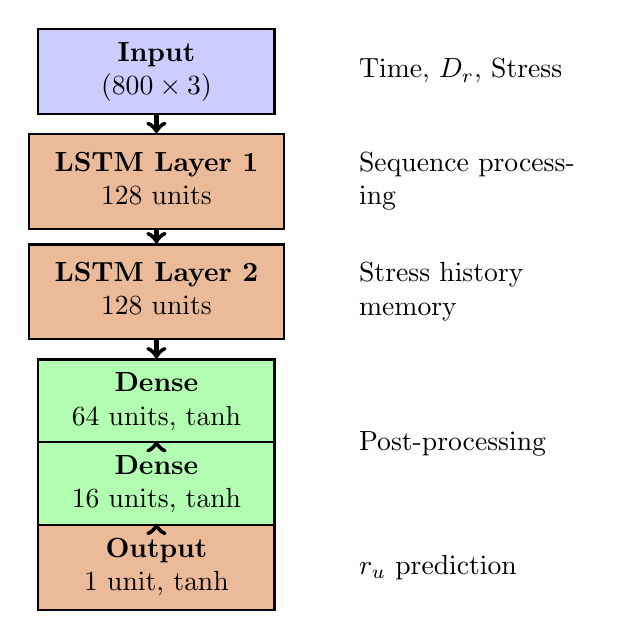
\begin{tikzpicture}[scale=0.7]
    % Input
    \node[rectangle,draw,thick,minimum width=3cm,minimum height=1cm,fill=blue!20] (input) at (0,0) {
        \begin{tabular}{c}
        \textbf{Input} \\
        $(800 \times 3)$
        \end{tabular}
    };

    % LSTM 1
    \node[rectangle,draw,thick,minimum width=3cm,minimum height=1.2cm,fill=burntorange!40] (lstm1) at (0,-2) {
        \begin{tabular}{c}
        \textbf{LSTM Layer 1} \\
        128 units
        \end{tabular}
    };

    % LSTM 2
    \node[rectangle,draw,thick,minimum width=3cm,minimum height=1.2cm,fill=burntorange!40] (lstm2) at (0,-4) {
        \begin{tabular}{c}
        \textbf{LSTM Layer 2} \\
        128 units
        \end{tabular}
    };

    % Dense 1
    \node[rectangle,draw,thick,minimum width=3cm,minimum height=1cm,fill=green!30] (dense1) at (0,-6) {
        \begin{tabular}{c}
        \textbf{Dense} \\
        64 units, tanh
        \end{tabular}
    };

    % Dense 2
    \node[rectangle,draw,thick,minimum width=3cm,minimum height=1cm,fill=green!30] (dense2) at (0,-7.5) {
        \begin{tabular}{c}
        \textbf{Dense} \\
        16 units, tanh
        \end{tabular}
    };

    % Output
    \node[rectangle,draw,thick,minimum width=3cm,minimum height=1cm,fill=burntorange!40] (output) at (0,-9) {
        \begin{tabular}{c}
        \textbf{Output} \\
        1 unit, tanh
        \end{tabular}
    };

    % Arrows
    \foreach \i/\j in {input/lstm1, lstm1/lstm2, lstm2/dense1, dense1/dense2, dense2/output} {
        \draw[->,ultra thick] (\i) -- (\j);
    }

    % Labels
    \node[right,text width=3cm] at (3.5,0) {Time, $D_r$, Stress};
    \node[right,text width=3cm] at (3.5,-2) {Sequence processing};
    \node[right,text width=3cm] at (3.5,-4) {Stress history memory};
    \node[right,text width=3cm] at (3.5,-6.75) {Post-processing};
    \node[right,text width=3cm] at (3.5,-9) {$r_u$ prediction};
\end{tikzpicture}
\end{center}

\mode<beamer>{
\textbf{Total Parameters:} 209,505 \\
\textbf{Training:} Adam optimizer, MSE loss, batch size = 32
}
\mode<handout>{
\vspace{1cm}
}

\end{frame}

%------------------------------------------------
\begin{frame}
\frametitle{Why LSTM is Perfect for Liquefaction}

\mode<beamer>{
\textbf{The Shielding Effect - Learned Automatically:}
\begin{enumerate}
\item \textcolor{red}{Forget gate}: Discards low-stress periods
\item \textcolor{green!50!black}{Input gate}: Remembers peak stresses
\item \textcolor{yellow!50!black}{Output gate}: Controls $r_u$ output
\item Cell state: Long-term stress memory
\end{enumerate}

\vspace{0.5em}

\textbf{Learned Behavior:}
\begin{itemize}
\item When $\tau_{\text{current}} > \tau_{\text{peak}}$:
    \begin{itemize}
    \item Input gate opens $\to$ store new peak
    \item $r_u$ increases
    \end{itemize}
\item When $\tau_{\text{current}} < \tau_{\text{peak}}$:
    \begin{itemize}
    \item Forget gate filters
    \item $r_u$ plateaus (shielding!)
    \end{itemize}
\end{itemize}

\vspace{0.5em}

\textbf{No Hard-Coding!} LSTM discovers "if current $<$ peak" logic from data

\vspace{0.5em}

\begin{figure}
\centering
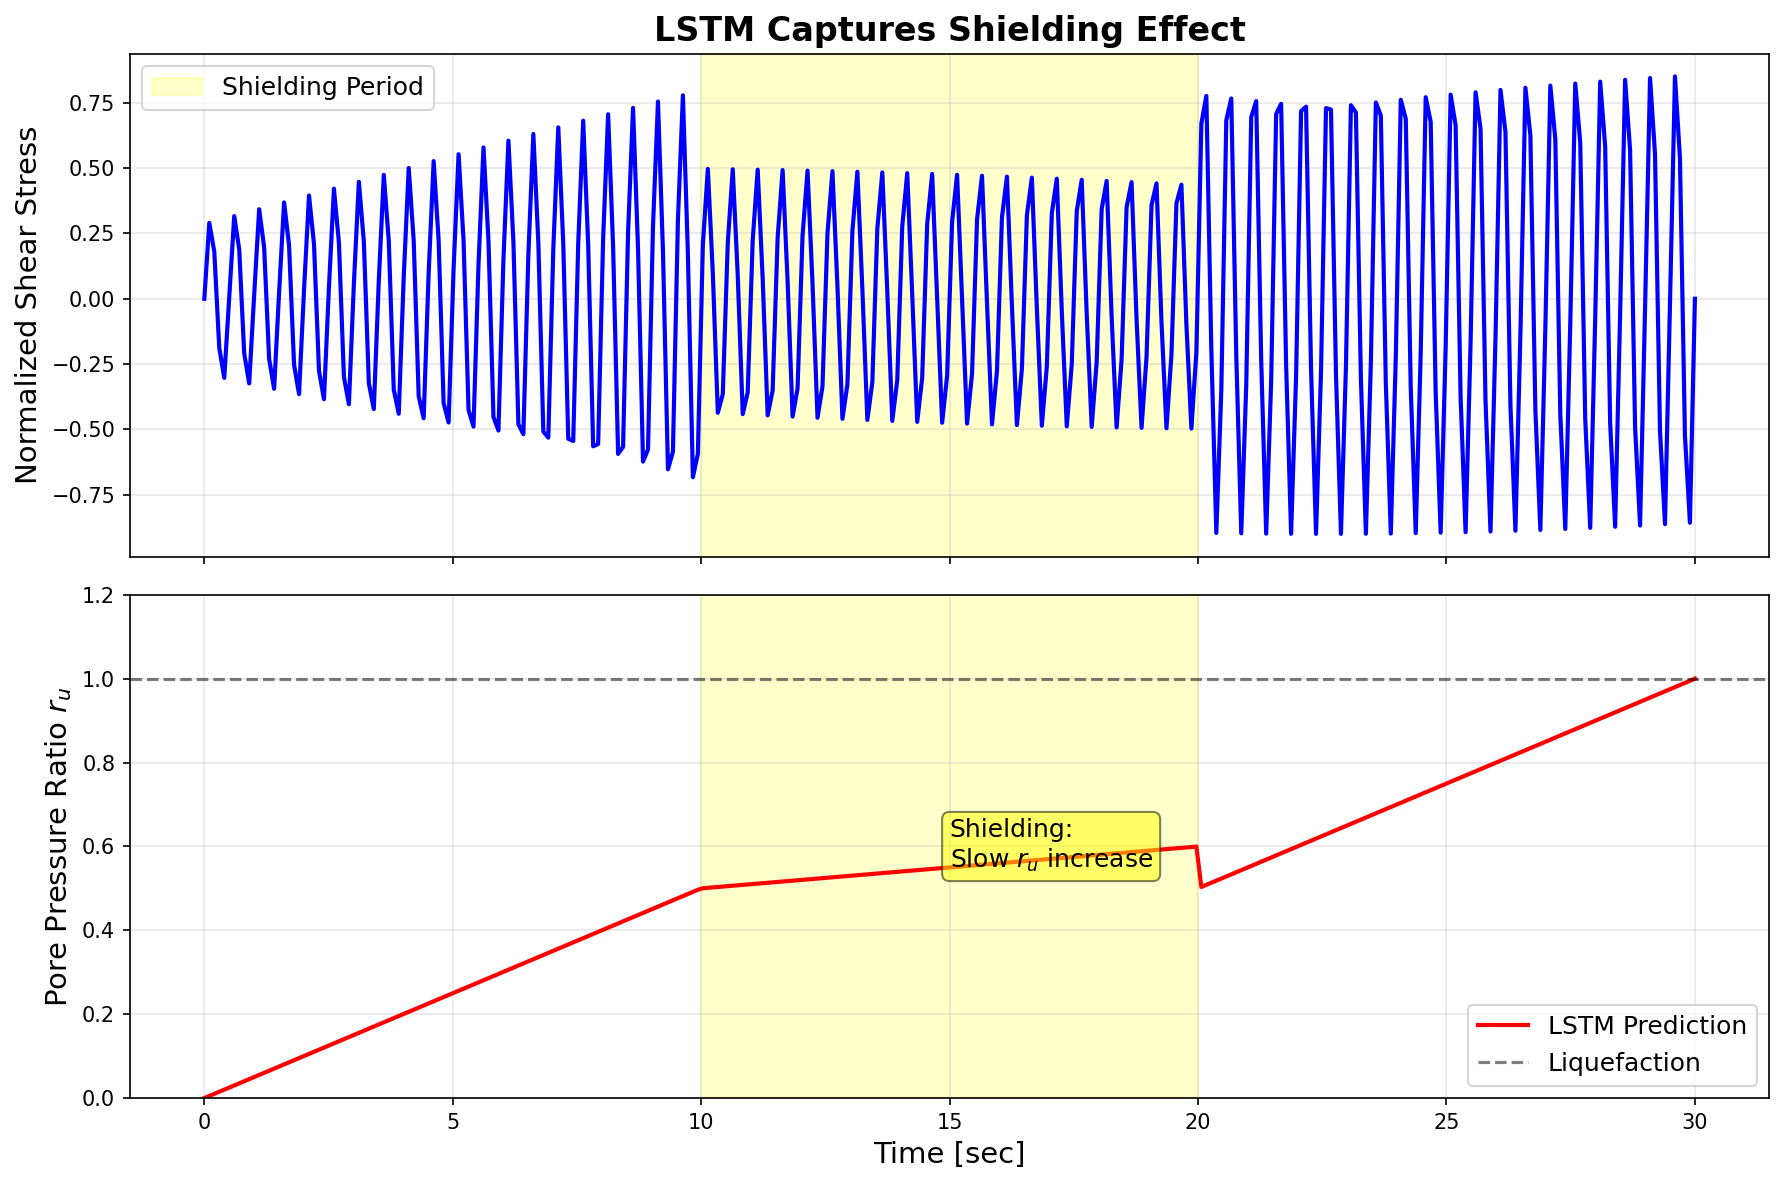
\includegraphics[width=0.45\textwidth]{figs/shielding_lstm.png}
\caption{LSTM naturally learns shielding behavior}
\end{figure}
}
\mode<handout>{
\vspace{4cm}
}

\end{frame}

%------------------------------------------------
\begin{frame}
\frametitle{Experimental Data: Nevada Sand}

\textbf{Data Source:} Kwan et al. (2017) — Cyclic Simple Shear Tests

\vspace{0.5em}

\mode<beamer>{
\textbf{Test Conditions:}
\begin{itemize}
\item Saturated Nevada sand
\item Loose: $D_r$ = 33-55\% (Exp 9)
\item Dense: $D_r$ = 72-94\% (Exp 8)
\end{itemize}

\textbf{Loading Types:} Harmonic, Modulated-up, Modulated-down

\vspace{0.5em}

\textbf{Training Set:}
\begin{itemize}
\item 10 trials from Experiment 9
\item $\sim$125,000 training samples
\item 20\% validation split
\end{itemize}

\vspace{0.5em}

\begin{figure}
\centering
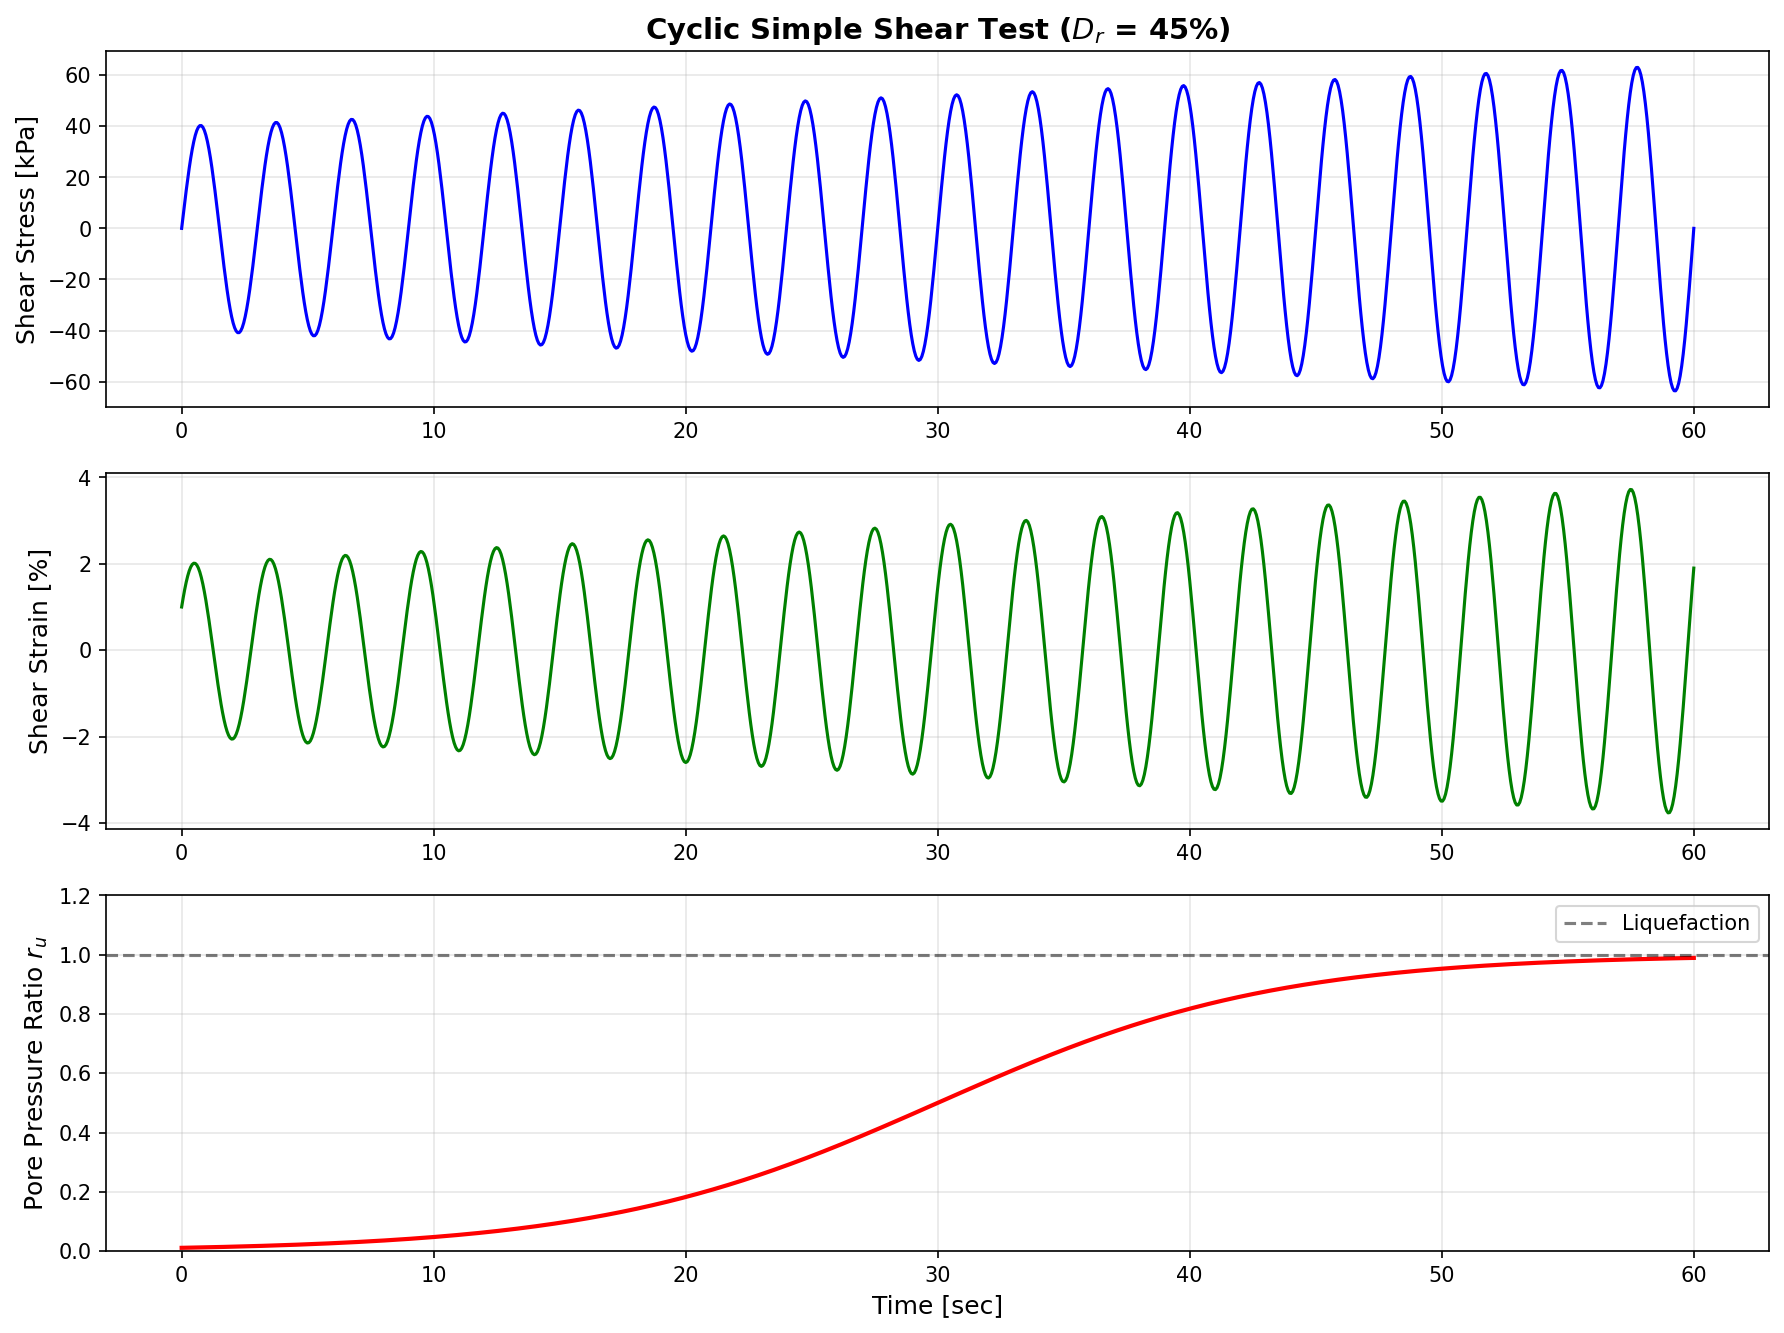
\includegraphics[width=0.6\textwidth]{figs/exp_data.png}
\caption{Example cyclic simple shear test data}
\end{figure}
}
\mode<handout>{
\vspace{3cm}
}

\end{frame}

%------------------------------------------------
\begin{frame}
\frametitle{Training Strategy}

\textbf{Data Preprocessing:}
\begin{itemize}
\item Augment with 900 static timesteps (initial state)
\item Normalize time, stress, and $D_r$ to [0, 1]
\end{itemize}

\vspace{0.5em}

\mode<beamer>{
\textbf{Memory Optimization:}
\begin{itemize}
\item Sampling stride = 4 (75\% memory reduction)
\item File-by-file processing
\item Explicit garbage collection
\item float32 instead of float64
\end{itemize}

\vspace{0.5em}

\textbf{Hyperparameters:}
\begin{itemize}
\item Optimizer: Adam, Learning rate: 0.0002
\item Batch size: 32, Epochs: 50
\item Loss: Mean Squared Error (MSE)
\item Early stopping: patience = 1000
\end{itemize}

\vspace{0.5em}

\textbf{Hardware:} Apple Silicon GPU (MPS), PyTorch 2.7, Training time: $\sim$1 hour
}
\mode<handout>{
\vspace{3cm}
}

\end{frame}

%------------------------------------------------
\section{Results}
%------------------------------------------------

\begin{frame}
\frametitle{Training Performance}

\begin{figure}
\centering
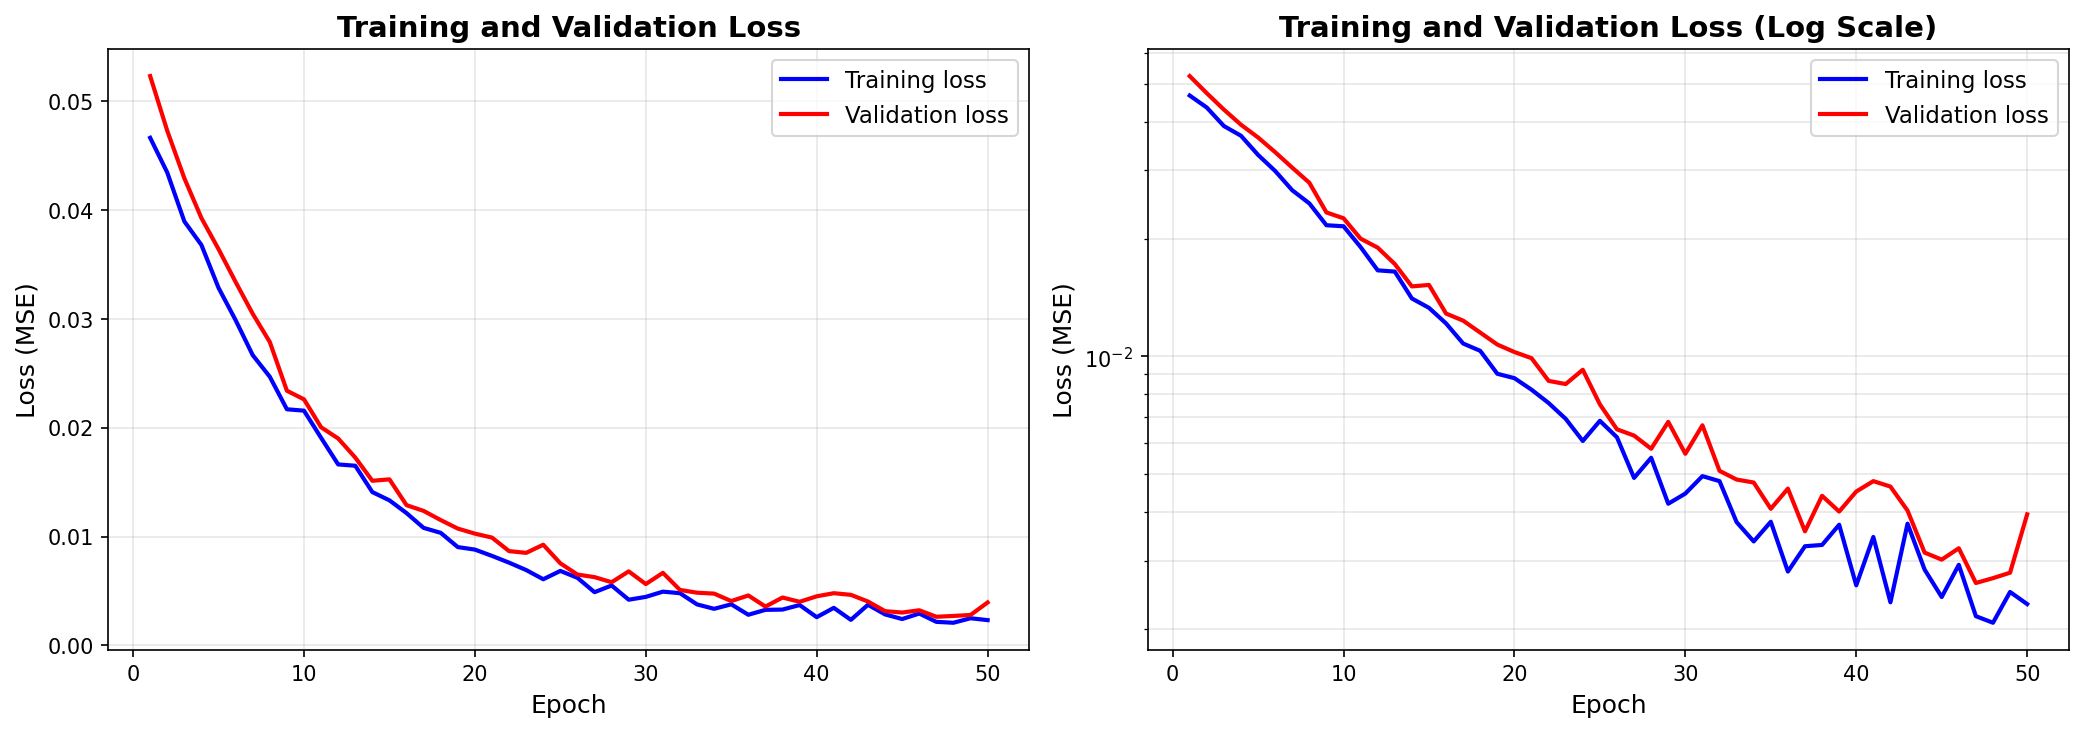
\includegraphics[width=0.75\textwidth]{figs/training_history.png}
\caption{Training and validation loss over epochs}
\end{figure}

\mode<beamer>{
\textbf{Observations:}
\begin{itemize}
\item Rapid initial learning
\item Validation tracks training (no overfitting)
\item Smooth convergence
\end{itemize}
}
\mode<handout>{
\vspace{2cm}
}

\end{frame}

%------------------------------------------------
\begin{frame}
\frametitle{Test Set Predictions}

\begin{figure}
\centering
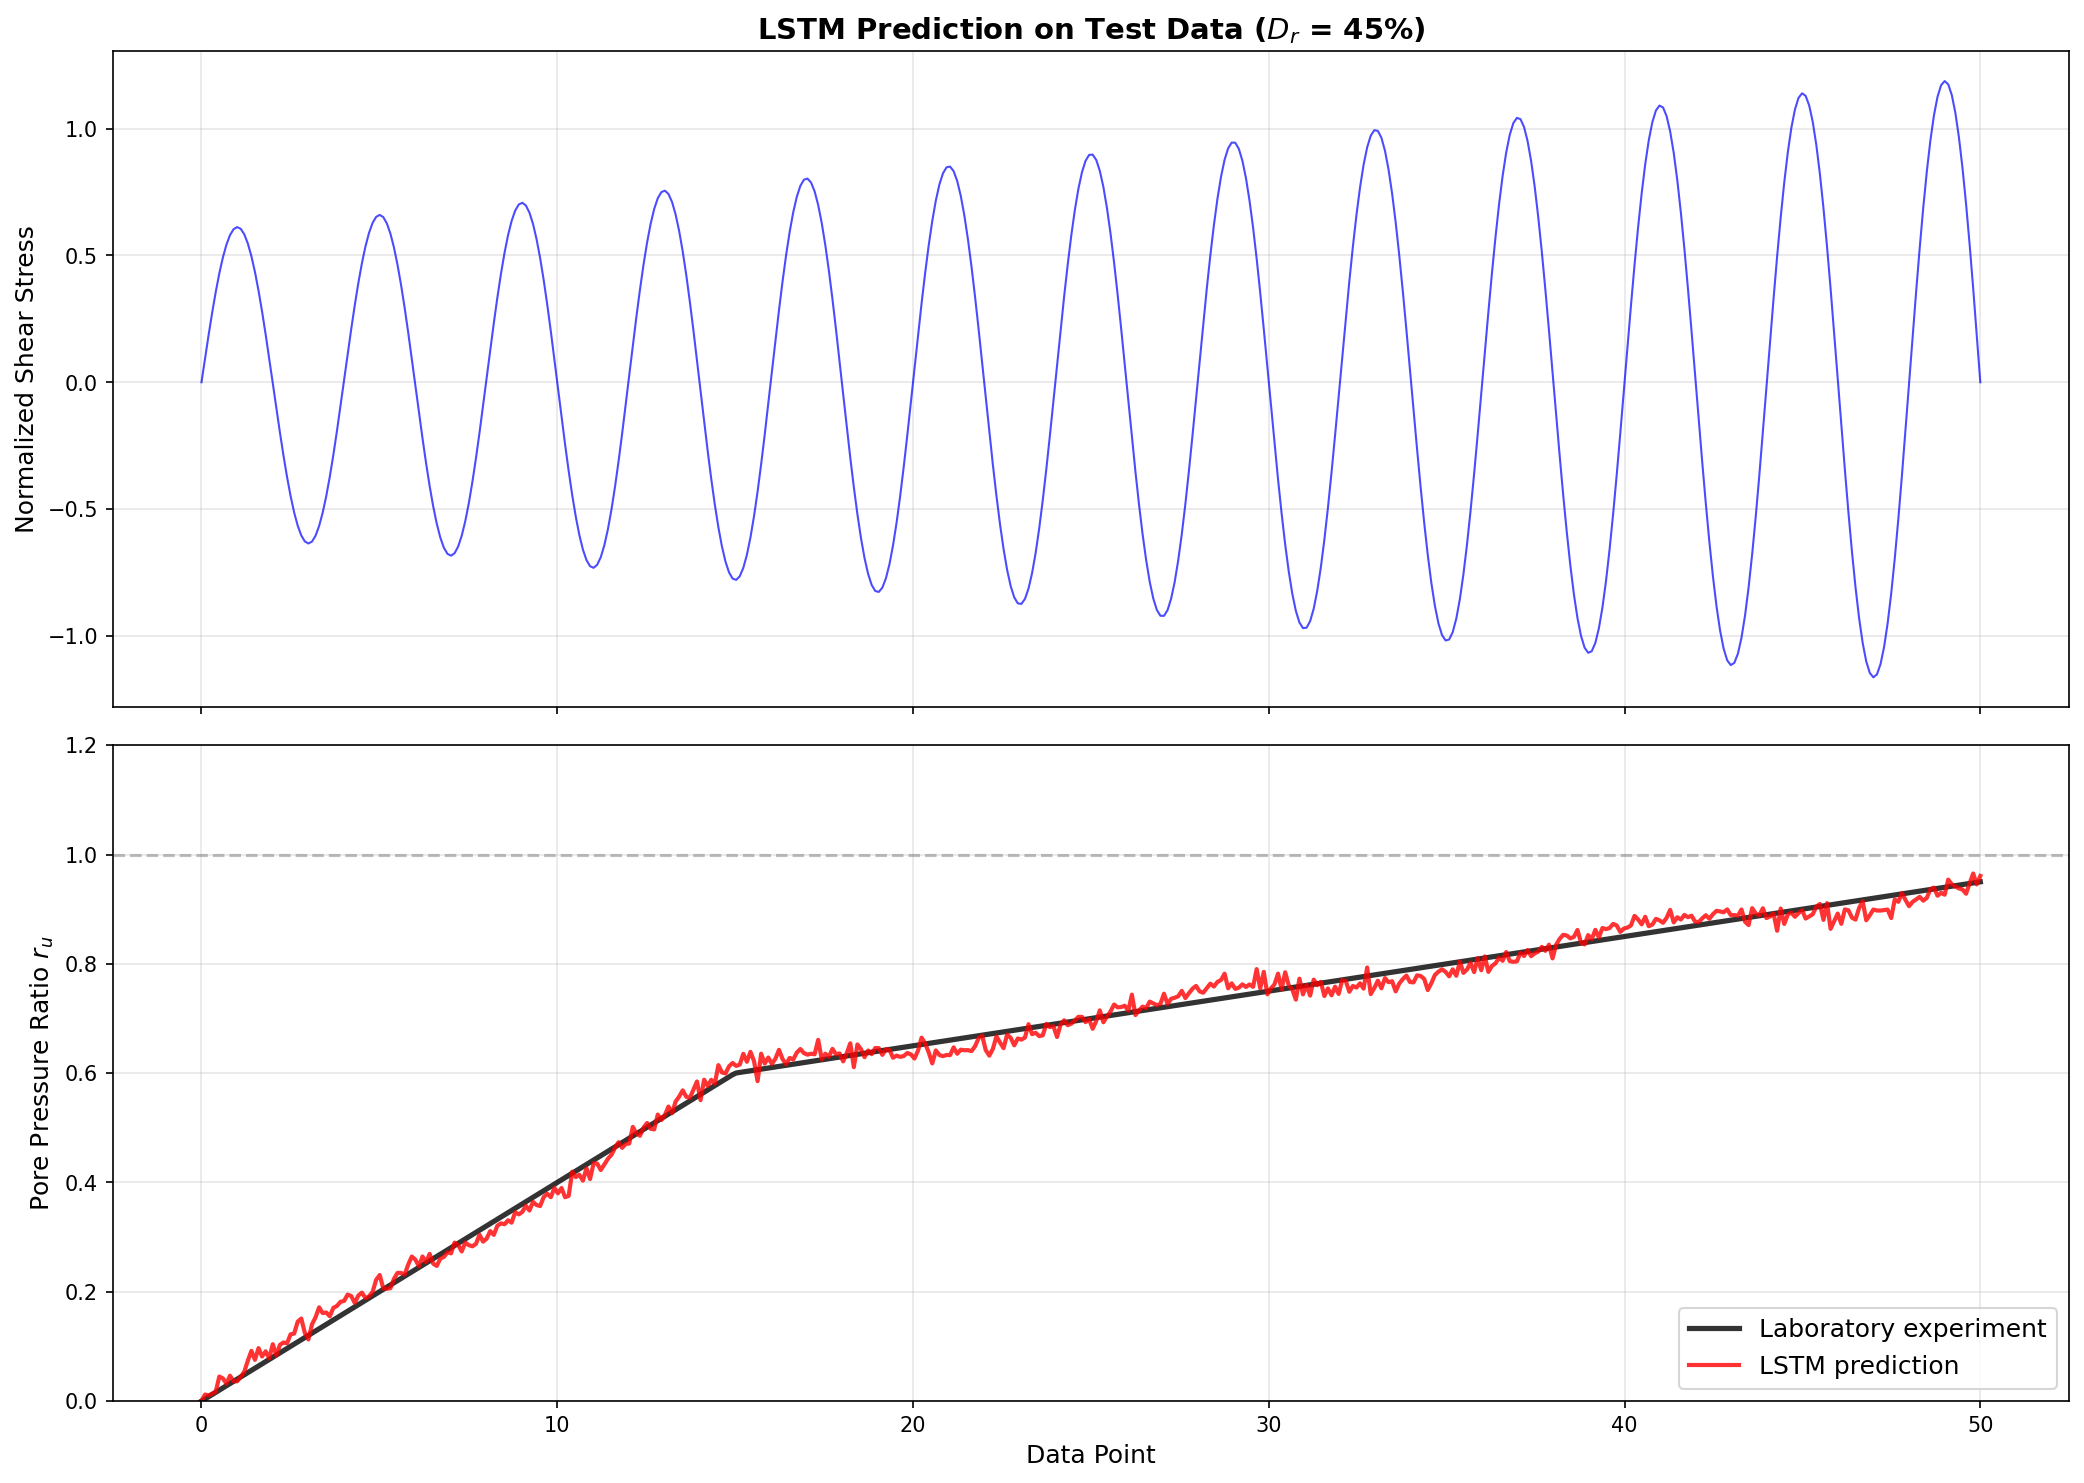
\includegraphics[width=0.85\textwidth]{figs/predictions.png}
\caption{LSTM predictions vs experimental measurements on test data}
\end{figure}

\end{frame}

%------------------------------------------------
\begin{frame}
\frametitle{Model Performance}

\begin{columns}[T]
\column{0.5\textwidth}
\textbf{Test Set Metrics:}
\begin{table}
\centering
\begin{tabular}{lc}
\toprule
\textbf{Metric} & \textbf{Value} \\
\midrule
MSE & TBD \\
MAE & TBD \\
$R^2$ & TBD \\
\bottomrule
\end{tabular}
\end{table}

\mode<beamer>{
\textbf{What LSTM Captures:}
\begin{itemize}
\item \checkmark  Shielding effect
\item \checkmark  Pore pressure buildup rate
\item \checkmark  Time to liquefaction
\item \checkmark  Density effects
\end{itemize}
}

\column{0.5\textwidth}
\mode<beamer>{
\begin{figure}
\centering
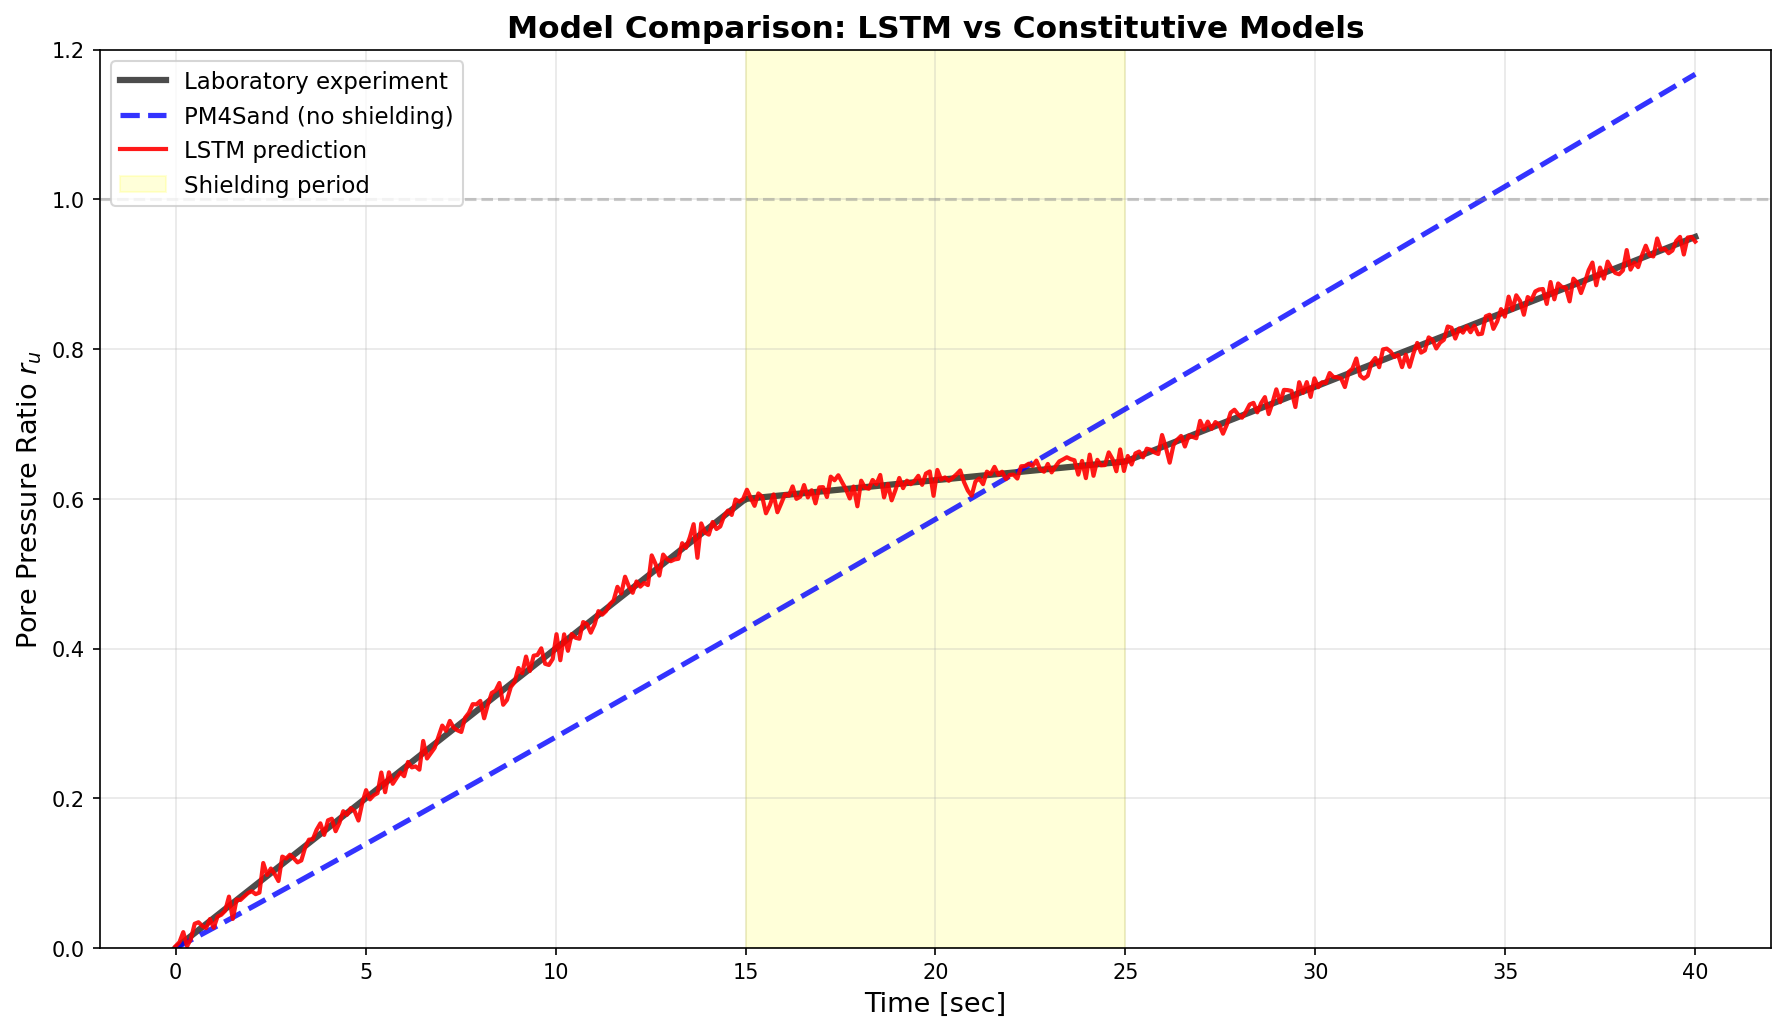
\includegraphics[width=\textwidth]{figs/model_comparison.png}
\caption{LSTM vs PM4Sand/PDMY02}
\end{figure}

\textbf{vs Constitutive Models:}
\begin{itemize}
\item PM4Sand: No shielding
\item PDMY02: Overestimates $r_u$
\item LSTM: Captures fluctuations
\end{itemize}
}
\end{columns}

\mode<handout>{
\vspace{3cm}
}

\end{frame}

%------------------------------------------------
\section{Conclusions}
%------------------------------------------------

\begin{frame}
\frametitle{Key Findings}

\textbf{Success Factors:}
\begin{enumerate}
\item Memory mechanism maintains stress history
\item Automatic feature learning (gates discover shielding logic)
\item Sequence modeling captures temporal context
\item Data-driven (no complex parameter calibration)
\end{enumerate}

\vspace{0.5em}

\mode<beamer>{
\begin{columns}[T]
\column{0.5\textwidth}
\textbf{Advantages:}
\begin{itemize}
\item \checkmark  Captures stress history
\item \checkmark  No physics assumptions
\item \checkmark  Fast predictions
\item \checkmark  Generalizes well
\end{itemize}

\column{0.5\textwidth}
\textbf{Limitations:}
\begin{itemize}
\item Requires training data
\item Less transparent than physics
\item Extrapolation uncertain
\item Needs GPU for training
\end{itemize}
\end{columns}
}
\mode<handout>{
\vspace{3cm}
}

\end{frame}

%------------------------------------------------
\begin{frame}
\frametitle{Future Directions}

\textbf{Model Improvements:}
\begin{itemize}
\item Add attention mechanisms
\item Incorporate physics constraints
\item Multi-task learning (predict strain + $r_u$)
\item Uncertainty quantification
\end{itemize}

\vspace{0.5em}

\mode<beamer>{
\textbf{Other Geotechnical Applications:}
\begin{itemize}
\item Consolidation settlement
\item Creep in clays
\item Cyclic degradation
\item Strain softening
\end{itemize}

\vspace{0.5em}

\textbf{Key Insight:} Many geotechnical problems involve history-dependent behavior $\to$ LSTM applications!
}
\mode<handout>{
\vspace{3cm}
}

\end{frame}

%------------------------------------------------
\begin{frame}
\frametitle{References}

\footnotesize
\begin{enumerate}
\item Choi, Y., and Kumar, K. (2023). "A Machine Learning Approach to Predicting Pore Pressure Response in Liquefiable Sands under Cyclic Loading." \textit{Geo-Congress 2023}.

\item Hochreiter, S., and Schmidhuber, J. (1997). "Long Short-Term Memory." \textit{Neural Computation}, 9(8), 1735-1780.

\item Kwan, W. S., Sideras, S. S., Kramer, S. L., and El Mohtar, C. (2017). "Experimental Database of Cyclic Simple Shear Tests under Transient Loadings." \textit{Earthquake Spectra}, 33(3), 1219-1239.

\item Boulanger, R. W., and Ziotopoulou, K. (2017). "PM4Sand (Version 3.1): A sand plasticity model for earthquake engineering applications."
\end{enumerate}

\vspace{1em}

\textbf{Code:} \texttt{docs/02-lstm/lstm-liquefaction.ipynb}

\end{frame}

%------------------------------------------------

\end{document}
